\documentclass{../UTNetLab}

\title{SDN and Nothing Else}
\authorshort{A. Khonsari, A. HajiAliKhamseh'i, M. Borhani, A. Khordadi, S. KashiPazha}
\author{%
    Dr. Ahmad Khonsari - \FR{دکتر احمد خونساری}\\
    \href{mailto:a_khonsari@ut.ac.ir}{a\_khonsari@ut.ac.ir}\\
    \vskip 1.5em%
    Amir Haji Ali Khamseh'i - \FR{امیر حاجی‌علی‌خمسه‌ء}\\
    \href{mailto:khamse@ut.ac.ir}{khamse@ut.ac.ir}\\
    \vskip 1.5em%
    \href{mailto:m.borhani@ut.ac.ir}{Muhammad Borhani} - \FR{محمد برهانی}\\
    \href{mailto:a.a.khordadi@ut.ac.ir}{Amirahmad Khordadi} - \FR{امیراحمد خردادی}\\
    \href{mailto:sina\_kashipazha@ut.ac.ir}{Sina Kashi pazha} - \FR{سینا کاشی‌پزها}
}

\begin{document}
    \selectlanguage{english}
    \maketitle

\section{SDN Introduction}
    \subsection{Excercise One}
    Remember previouse lab \footnote{Lab 4 routing} where you are using host rather than router to emulate some routing functionality. In this experiment we want to implement same functionality with SDN switches. To warm up our hands we will start by simple scenario:

    \begin{itemize}
    	\setlength{\itemindent}{10pt}
    	\item Open switch.py and read it's codes carfully.
    	\item Run this code with \textbf{sudo python switch.py}
    	\item Ping h2 from h1.
    	\item Capture OpenFlow hello packet on \textbf{lo} interface. (Filter wireshark output with \textbf{of} filter)
    \end{itemize}

    \subsubsection*{Lab Report}
    \begin{itemize}
    	\setlength{\itemindent}{0pt}
    	\item Expain line 21 to 26 of switch.py.
    	\item Read \href{http://flowgrammable.org/sdn/openflow/state-machine/}{this link} and explain switch handshak with controller. What is xid of your packets. Justify your answer with captured packets. \textbf{Don't copy and paste text from refrence in your lab report}.
    \end{itemize}

    \subsection{Excercise Two}
    Use what you learned in previouse exercise and create figure \ref{fig:linearRouters} topology. Configure switches in this topology where ??? we can ping each host from each host. Show your final result to instructors.

    \begin{figure}[H]
    	\centering
    	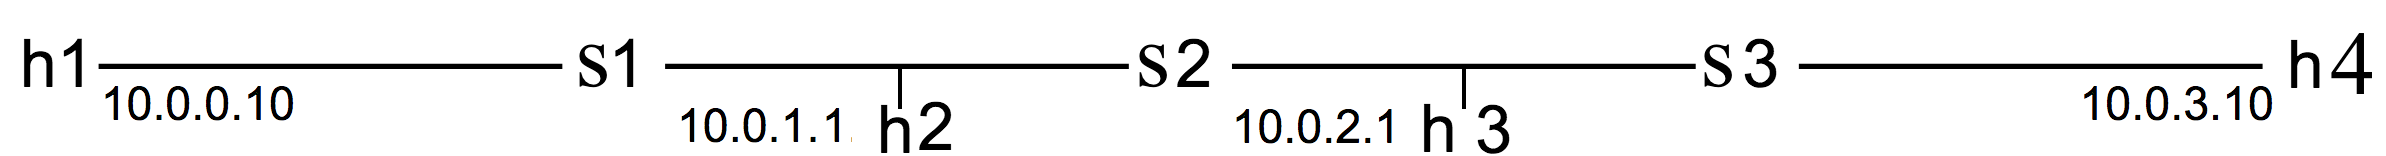
\includegraphics[height=30pt]{img/fig1.png}
    	\caption{Mininet Topology}
    	\label{fig:linearRouters}
    \end{figure}


\section{Exercises with multitables flows}
    \subsection*{Excercise Three}
    In this section we are loading switch flows from another files and axamining it's functionality.

    \begin{itemize}
    	\setlength{\itemindent}{10pt}
    	\item Execute \textbf{sudo python topo.py} 
    	\item Execute \textbf{sh ovs-ofctl add-flows s1 tables.txt} on mininet console.
    	\item Ping each host from other hosts.
    	\item Capture ICMP packets on each host and observe network behavior.
    	\item Modify tables.txt to drop packets between h1 and h2.
    \end{itemize}

    \begin{figure}[H]
    	\centering
    	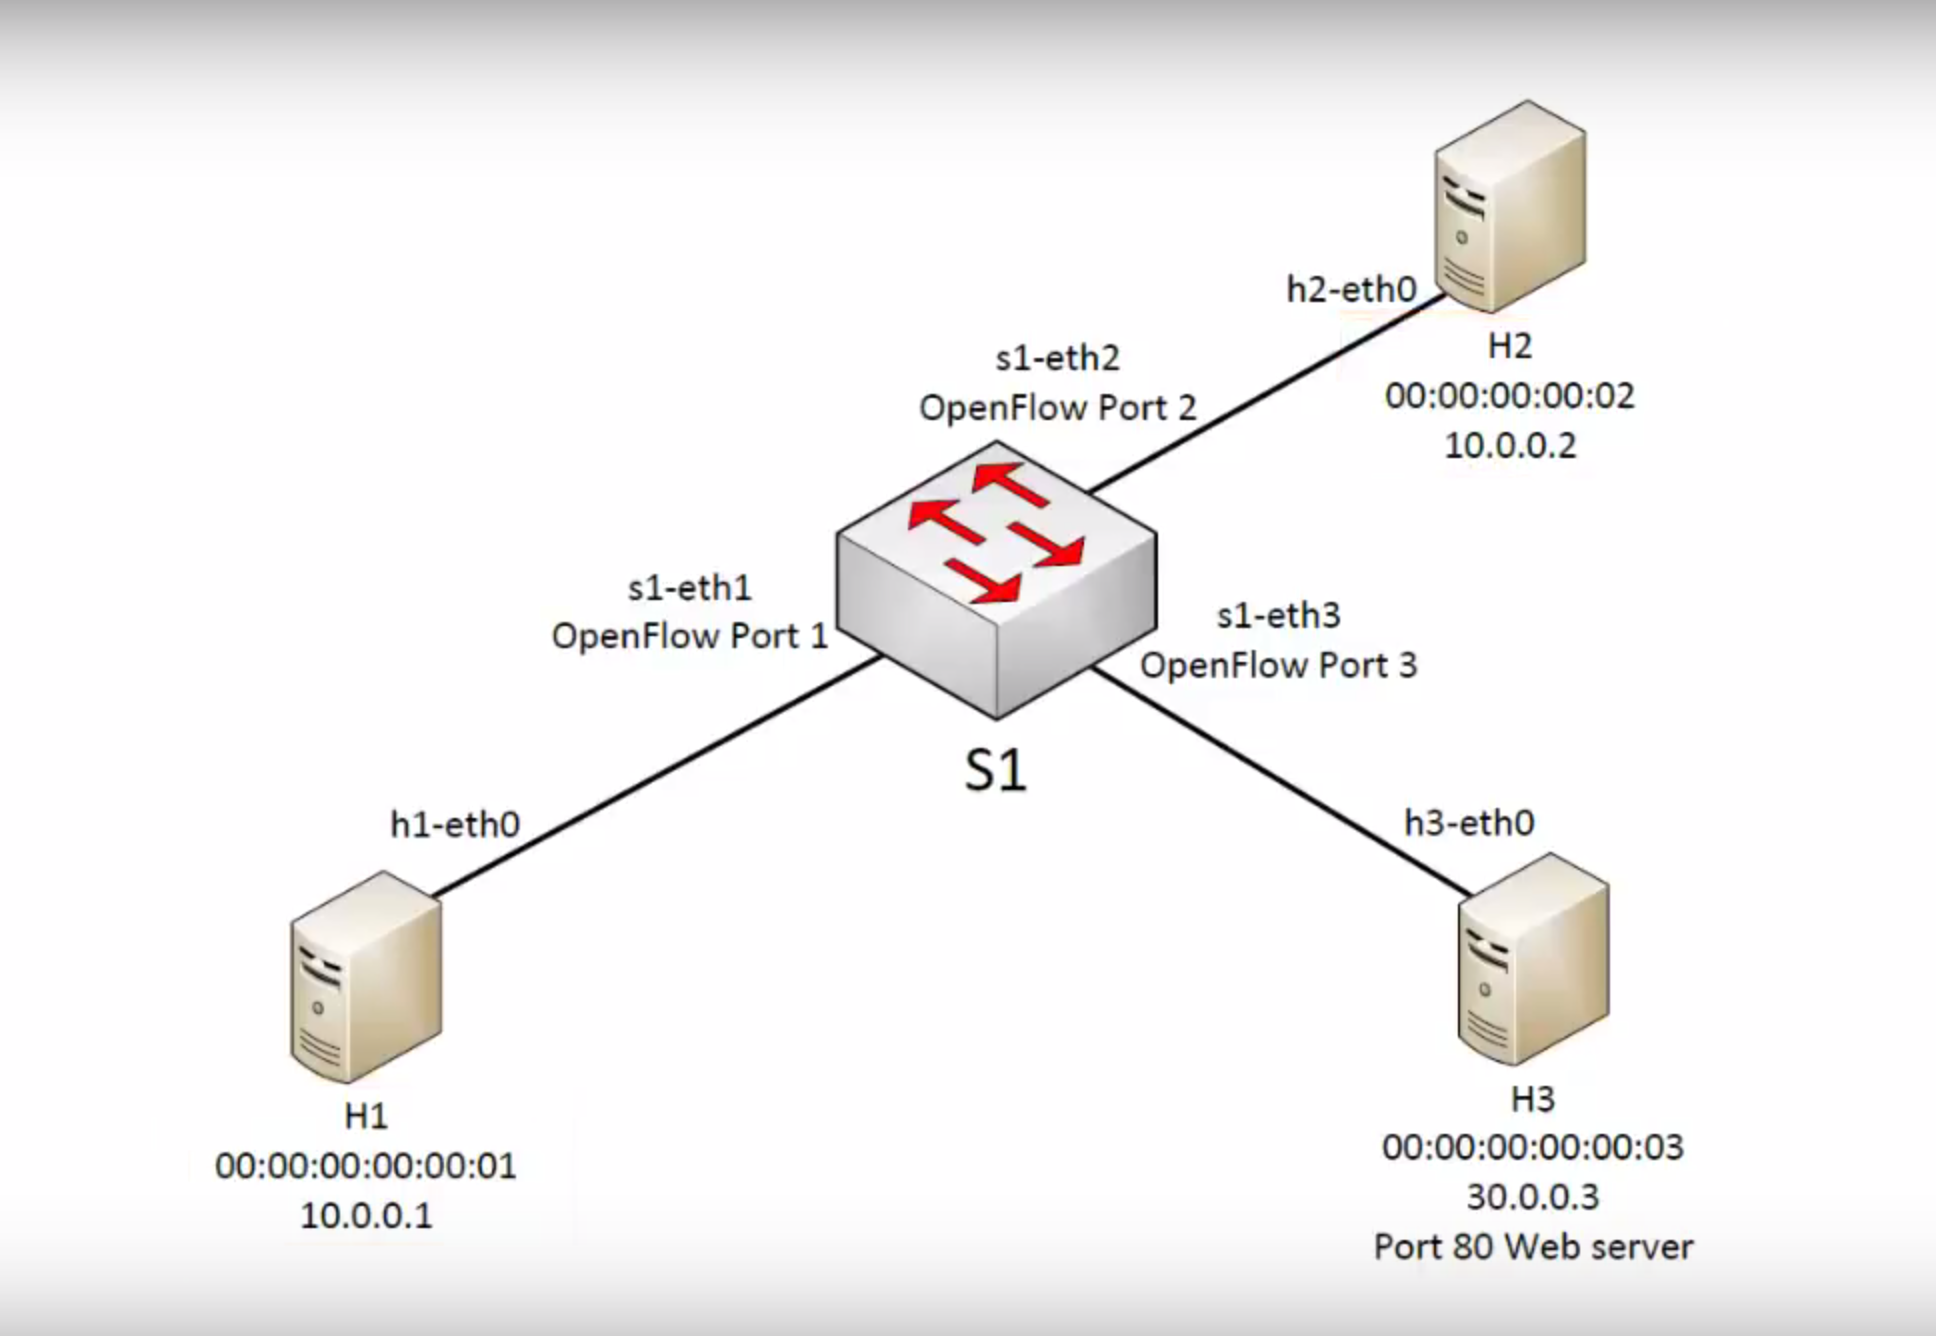
\includegraphics[height=300pt]{img/fig2.png}
    	\caption{Multi Table Scenario}
    	\label{fig:MultiTableScenario}
    \end{figure}


    \subsubsection*{Lab Report}
    \begin{itemize}
    	\setlength{\itemindent}{0pt}
    	\item Can you explain switch behavior? Justify your answer with wireshark output and tables.txt file.
    \end{itemize}
\end{document}
